\lstinputlisting[style=cstyle]{Questions/Part4/prime4.c}

\subsubsection*{\underline{Experimental}}

\begin{tabular}{|c|c|c|c|c|c|c|c|c|c|c|}
\hline
N & 1000003 & 2000003 & 4000037 & 8000009 & 16000057 & 32000011 & 64000031 & 128000003 & 256000001 & 512000009 \\
\hline
\makecell{T(n)\\\(10^{-5}\)} & 6.5 & 7.4 & 7.5 & 7.8 & 8.5 & 8.7 & 11.2 & 11.4 & 13.8 & 14.5\\
\hline
\end{tabular}

\vspace{0.25cm}

\begin{tabular}{|c|c|c|}
    \hline
    N & 1024000009 & 2048000011\\
    \hline
    \makecell{T(n)\\\(10^{-5}\)}  & 17.1 & 19\\
    \hline
\end{tabular}



\vspace{0.5cm}

\begin{figure}[h!]
    \centering
    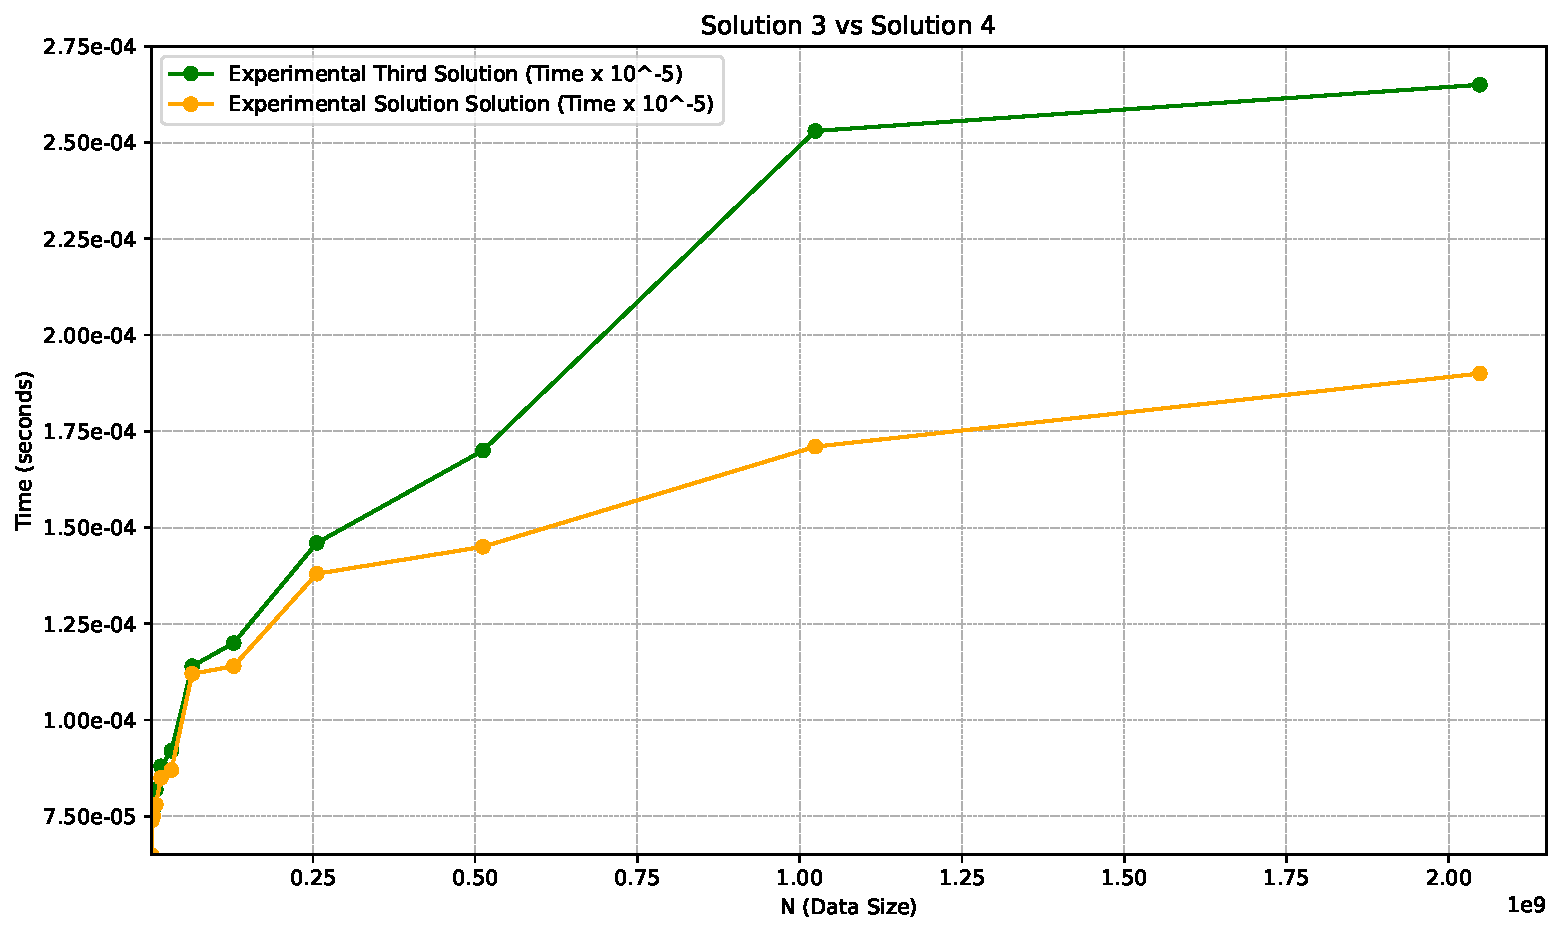
\includegraphics[width=0.85\textwidth]{Questions/Part4/plot.pdf}
    \label{fig:time_plot}
\end{figure}

\newpage

To Draw the plots i used the below python script :

\vspace{1cm}

\lstinputlisting[style=pythonstyle2,inputencoding=utf8]{Questions/Part4/draw.py}

\vspace{1cm}

\begin{prettyBox}{Observation}{greenPlot}
From the plots we notice that the 4th solution takes about the same time as 3rd solution but as n grows bigger the 4th solution takes about
half time of the 3rd therefore the 4th solution is the most efficient out of all the solutions
\end{prettyBox}


